\chapter{Background}\label{ch2}

Lorem ipsum dolor sit amet, consectetur adipiscing elit,
sed do eiusmod tempor incididunt ut labore et dolore magna aliqua.
Ut enim ad minim veniam, quis nostrud exercitation ullamco laboris nisi ut aliquip ex ea commodo consequat.
Duis aute irure dolor in reprehenderit in voluptate velit esse cillum dolore eu fugiat nulla pariatur.
Excepteur sint occaecat cupidatat non proident, sunt in culpa qui officia deserunt mollit anim id est laborum.

\section{My Section}

A paragraph refer to another section, see section \ref{other_sec} for details.

Lorem ipsum dolor sit amet, consectetur adipiscing elit,
sed do eiusmod tempor incididunt ut labore et dolore magna aliqua.
Ut enim ad minim veniam, quis nostrud exercitation ullamco laboris nisi ut aliquip ex ea commodo consequat.
Duis aute irure dolor in reprehenderit in voluptate velit esse cillum dolore eu fugiat nulla pariatur.
Excepteur sint occaecat cupidatat non proident, sunt in culpa qui officia deserunt mollit anim id est laborum.

Lorem ipsum dolor sit amet, consectetur adipiscing elit,
sed do eiusmod tempor incididunt ut labore et dolore magna aliqua.
Ut enim ad minim veniam, quis nostrud exercitation ullamco laboris nisi ut aliquip ex ea commodo consequat.
Duis aute irure dolor in reprehenderit in voluptate velit esse cillum dolore eu fugiat nulla pariatur.
Excepteur sint occaecat cupidatat non proident, sunt in culpa qui officia deserunt mollit anim id est laborum.


\section{My other section}\label{other_sec}

See formual \ref{eq:domain} and \ref{eq:softmax}

Lorem ipsum dolor sit amet, consectetur adipiscing elit,
sed do eiusmod tempor incididunt ut labore et dolore magna aliqua.
Ut enim ad minim veniam, quis nostrud exercitation ullamco laboris nisi ut aliquip ex ea commodo consequat.
Duis aute irure dolor in reprehenderit in voluptate velit esse cillum dolore eu fugiat nulla pariatur.
Excepteur sint occaecat cupidatat non proident, sunt in culpa qui officia deserunt mollit anim id est laborum.

\begin{equation}\label{eq:domain}
D = \{ \chi , P(X) ; X \in \chi \}
\end{equation}

and given a labeled training dataset \( T = \{ (X_1, y_1), (X_2, y_2), ... \} \),
for \( X_i \in \chi \), \( y_i \in Y \).

The classification task is defined\autocite{pan2010survey} to find a function \( g(X) \) that predicts the label
having maximum conditional probability \( P(y|x) \) 
or predict the joint probability of each label \( f(X,y) = P(X,y) \) in the domain

\begin{equation}
softmax(o_j) = \frac{e^{o_j}}{ \sum\limits_{i=1}^n e^{o_i} }
\label{eq:softmax}
\end{equation}

See figure \ref{fig:regularization} and \ref{fig:resnet} to see how we insert graphs.
Also one can refer sub-figure as in figure \ref{fig:resnet-block}.
All those were EPS, PDF and SVG using ``save as'' feature in Inkscape.
And for tables, see table \ref{table:inception-ver-1-4}.

\begin{table*}\caption{Comparing all versions of Inception}\label{table:inception-ver-1-4}
\centering
\begin{tabular}{@{}cccccc@{}}
\toprule
Model Name & layers & weights & mults & Top-1 accuracy & Top-5 accuracy \\
\midrule
Inception v1 & 22 & 6.6M & 1,498M & 69.8 & 89.6 \\
Inception v2 & 42 & 11M & 1,934M & 73.9 & 91.8 \\
Inception v3 & 53 & 27M & 5,719M & 78.0 & 93.9 \\
Inception v4 & 81 & 46M & 13,882M & 80.2 & 95.2 \\
Inception ResNet V2 & 130 & 59M & 14,882M & 80.4 & 95.3 \\
\bottomrule
\end{tabular}
\end{table*}



Lorem ipsum dolor sit amet, consectetur adipiscing elit,
sed do eiusmod tempor incididunt ut labore et dolore magna aliqua.
Ut enim ad minim veniam, quis nostrud exercitation ullamco laboris nisi ut aliquip ex ea commodo consequat.
Duis aute irure dolor in reprehenderit in voluptate velit esse cillum dolore eu fugiat nulla pariatur.
Excepteur sint occaecat cupidatat non proident, sunt in culpa qui officia deserunt mollit anim id est laborum.

\begin{figure}[!h]
\centering
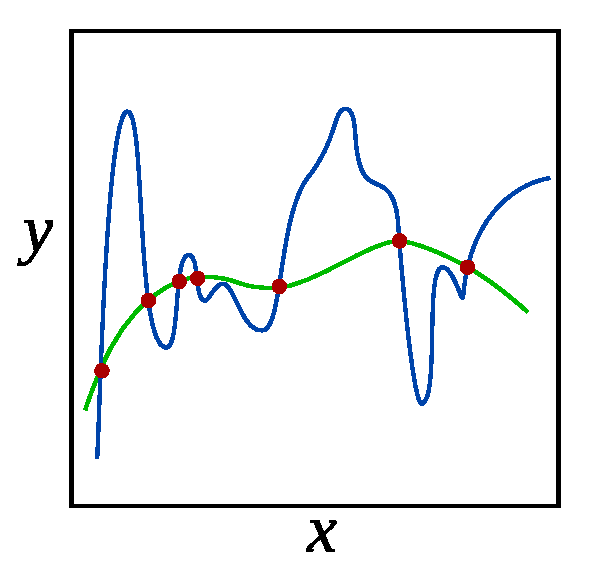
\includegraphics[width=2in]{regularization}
\caption{Two curves that have same loss of zero. Green one have smaller weights, blue one have higher weights. }\label{fig:regularization}
{Source: \href{https://commons.wikimedia.org/wiki/File:Regularization.svg}{Wikipedia}\hfill}
\end{figure}


\begin{figure}[!h]
\centering
    \begin{subfigure}[b]{0.4\textwidth}
        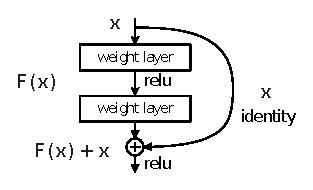
\includegraphics[width=\textwidth]{resnet}
        \caption{ResNet Building Block}\label{fig:resnet-block}
    \end{subfigure}
    \begin{subfigure}[b]{0.4\textwidth}
        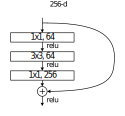
\includegraphics[width=\textwidth]{resnet-bottleneck}
        \caption{ResNet Bottleneck}\label{fig:resnet-bottleneck}
    \end{subfigure}
\caption{ResNet building block blah blah blah blah blah blah.}\label{fig:resnet}
{Source: \cite{he2016deep}\hfill}
\end{figure}


One can also refer to raster images as in figure \ref{fig:birds200}

\begin{figure}[!h]
\centering
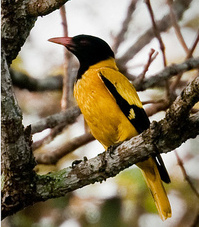
\includegraphics[width=2in]{birds200-hooded-oriole}
\caption{A bird picture from birds-200 database.}\label{fig:birds200}
{Source: \cite{WahCUB_200_2011}\hfill}
\end{figure}
